\section{The LSST Camera (LSSTCam)} \label{sec:lsstcam}

% Biblio
The Vera C. Rubin Observatory's camera LSSTCam (https://lsstcam.lsst.io/) is the largest digital camera ever built to date.
Its design and and the technological progress it required, were developed in order to meet the requirements set by the ambitious goals of LSST, as described in \textcolor{red}{add citation to LSST Camera Verification Testing and Characterization and other SPIE papers}).
We have thus created an ISR approach specifically for the analysis of LSSTCam images.
Figure \ref{fig:beforeafterISR} shows an example of the results form our ISR pipeline on an LSSTCam exposure, showing the corrections of large effects (such as the amplifier offset or crosstalk) as well as more subtle effects (such as the brighter fatter effect).
We summarize here key points about LSSTCam and properties of its CCDs relevant for LSSTCam calibration in Rubin Data Management (DM).


\begin{figure*}[t]
    \centering
    % TODO: add before/after ISR figure asset
    \fbox{\parbox{0.75\textwidth}{\centering\vspace{1.5in}\small\textit{Figure pending}\vspace{1.5in}}}
    \caption{Here is an exposure before and after ISR.
    }
    \label{fig:beforeafterISR}
\end{figure*}


\subsection{LSSTCam CCDs} \label{sec:data:lsstcam}

% Focal plane
LSSTCam, is composed of 189 CCDs organized in rafts of 9 CCDs (3x3), in a focal plane mosaic presented in CTN-001 \textcolor{red}{add citation}.
In addition, 2 star guider CCDs and one split-wavefront CCD are at each four corners of the focal plane mosaic.
We will focus only on the science CCDs in the following as no requirements are set on the calibration of the corner sensors within DM, although some calibrations are provided for the star guiders.

% CCDs
LSSTCam CCDs are made of 16 segments each, 8 at the top and 8 at the bottom of the CCD, read out through an amplifier.
Segments are commonly referred to as amplifiers and will be in the rest of this paper.
Each amplifier is 2048 pixels high and 512 pixels wide for e2v and \textcolor{red}{add ITL case}.
Figure \ref{fig:amplifier} shows a diagram of the amplifier geometry and direction of electrons transportation in LSSTCam CCDs.
%here add more about electron transportation and size of ovescan region and serial register.
The overscan regions are virtual pixels read to estimate charge transfer inefficiency (CTI), see \ref{sec:processing:calibration:cti} for my details.
Figure \ref{fig:amplifier} show an example of the signal read in the overscan region for ITL and e2v amplifiers.

\begin{figure*}[t]
    \centering
    % TODO: add amplifier geometry figure asset
    \fbox{\parbox{0.75\textwidth}{\centering\vspace{1.5in}\small\textit{Figure pending}\vspace{1.5in}}}
    \caption{Here is an exposure in e2v amplifier and in ITL amplifier with rectangles around different regions (overscans, serial register)
    and graphs of the signal in their overscan regions.
    }
    \label{fig:amplifier}
\end{figure*}


\subsection{Electronic Detector Model for LSSTCam} \label{sec:lsstcam:detector-model}

We have built on the ISR approach of past optical surveys \textcolor{red}{here add citations for ISR procedures for other CCD optical experiments}
to develop an ISR pipeline specifically designed for LSSTCam.
At Calibpalooza 2022 (\textcolor{red}{is their proceeding or document we can refer to?}) and during following years,
we have indeed defined the electronic model of LSSTCam and associated effects in the photon to ADU signal chain.
Figure \ref{fig:detector-boxes} depicts the different steps in this chain and their physical ordering from the detector
to the Readout Board (REB). \textcolor{red}{here add any citations that supports this description.}
%Figure~\ref{fig:detector-boxes} summarizes the instrumental effects identified in the photon transfer chain and their order.

The ISR pipeline implemented in the Rubin data processing aims at correcting each of these effects in the order opposite to which they happen.

\begin{figure*}[t]
    \centering
    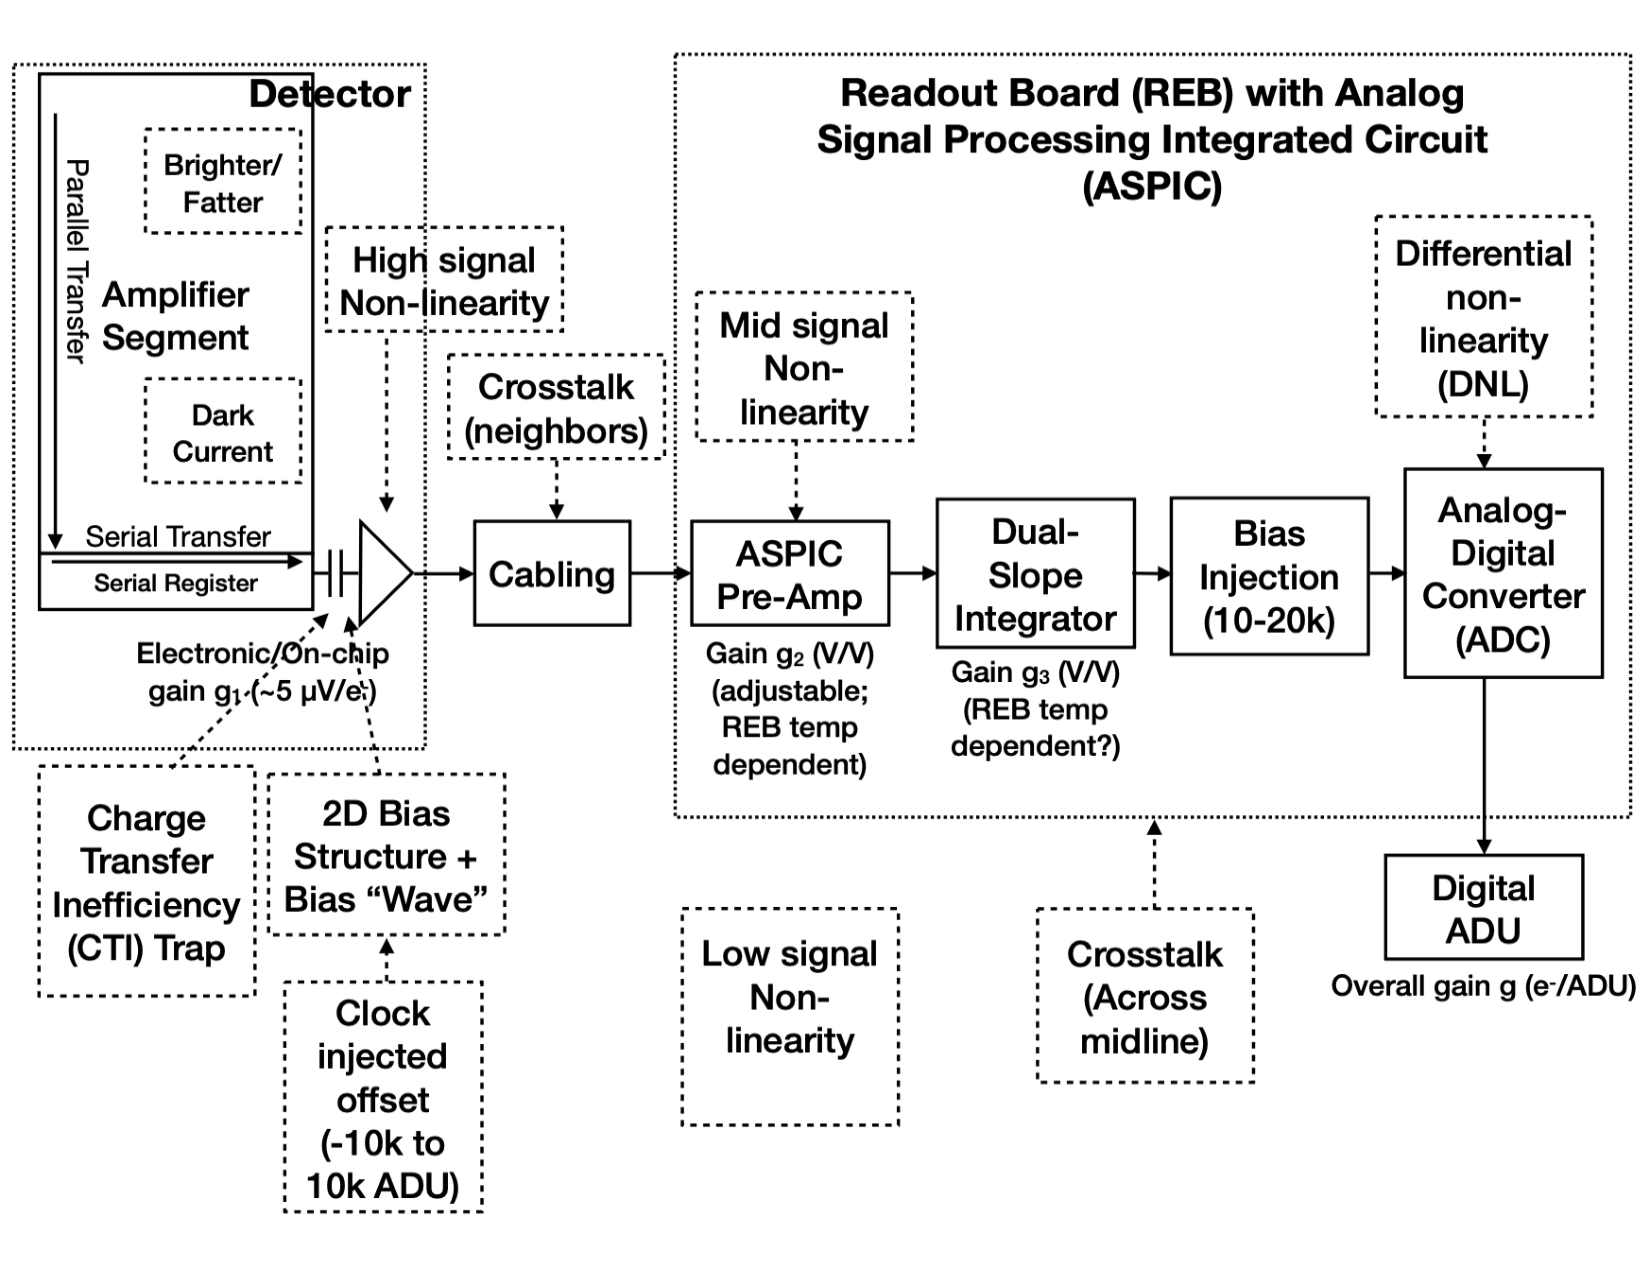
\includegraphics[width=0.8\textwidth]{figures/calibration_boxes_detector_model.pdf}
    \caption{Photon transfer and data-acquisition model for the LSSTCam detectors and electronic readout board (REB).
    Instrumental effects seen in images are shown as dashed boxes; arrows indicate where each effect enters the chain.
    Low-signal nonlinearities in LSSTCam's detector response have been observed, but their origin is not yet established; that contribution appears as a disconnected box.}
    \label{fig:detector-boxes}
\end{figure*}

